\section{Aufbau von Ludimus (ES)}
\subsection{Übersicht}

Ludimus selbst ist in zwei Applikationen unterteilt. Eine läuft auf einem Gerät welches man als Controller benutzten will,
dies kann ein Smartphone oder ein anderes Gerät, auf welchem Android lauft, sein und eine Applikation welche auf einem Laptop, PC, Tablet oder SmartTV läuft. Diese wird ab sofort als Server bezeichnet.
Der User muss dann auf seinem Controller einen Code eingeben oder scannen mit welchem sich das Gerät dann zu der Anwendung welche auf dem Server läuft verbindet. Der User bedient nach dem Aufbau der Verbindung die komplette Plattform mit seinem Controller. Die Verbindung ist in der Abbildung \ref{img:Ablauf} nochmal deutlicher dargestellt. 
\begin{figure}
    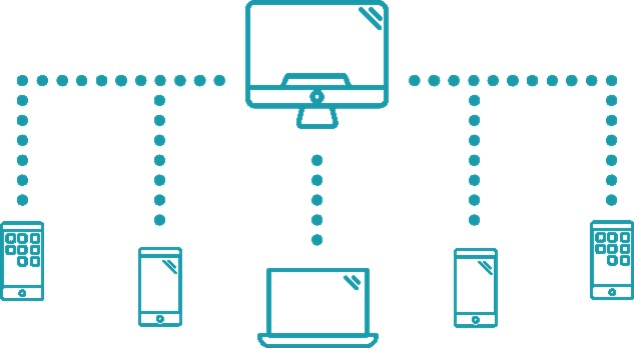
\includegraphics[scale=0.6]{images/ludi.jpg}
    \caption{Aufbau Ludimus}
    \label{img:Aufbau}
\end{figure}
\pagebreak
\subsection{Ablaufdiagram Ludimus}
\begin{figure}
    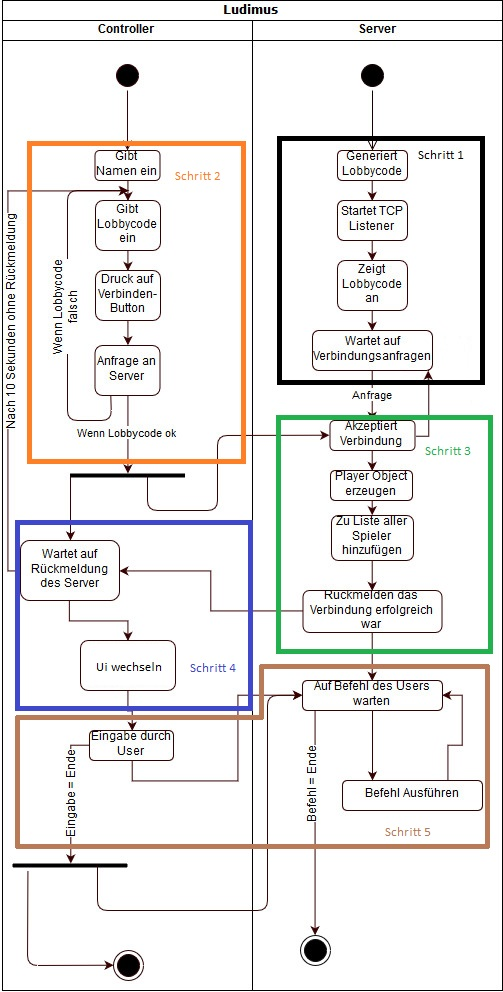
\includegraphics[scale=1.5]{images/Sequence1.jpg}
    \caption{Ablaufdiagram Ludimus}
    \label{img:Ablauf}
\end{figure}
\subsubsection{Erklärung des Ablaufdiagrams(\ref{img:Ablauf})}
\paragraph{Schritt 1}
Im ersten Schritt generiert der Server zunächst einen Lobbycode aufgrund der IP-Adresse des Gerätes.
Genauer ist dies im Kapitel Lobbycodes \ref{lobbycodes} beschrieben. Danach öffnet der Server den TCP Listener, dies sieht im Code so aus:
\newline \textit{ this.listener = new TcpListener(IPAddress.Parse(this.ipAdress), 9393);\newline
this.listener.Start();}\newline
Wichtig ist hierbei das der TCPListener auch noch gestartet werden muss nach der Erzeugung. Mehr dazu im Kapitel \ref{tcplistener}.
Wenn der TCP Listener erfolgreich gestartet wurde kann der Lobbycode auch angezeigt werden, da ab nun sich Spieler verbinden können. Im Code wird das so realisiert: \newline
\textit{this.LobbyCodeText.text = "Lobbycode: " + this.playermanager.GetLobbyCode();}\newline
Wobei dies in der Initialisierung des UI's und sommit in einer anderen Klasse geschiet. Deshalb wird hier auch die
\textit{GetLobbyCode()} Methode des Playermanagers verwendet. \textit{this.LobbyCodeText} ist das TextElement welches in Unity erzeugt wurde.
Letzter Teil dieses Schrittes besteht darin den TCP Listener „horchen“ zu lassen, damit er auch auf die Anfragen reagieren kann. Code: \newline
\textit{ var tmpClient = this.listener.AcceptTcpClient();} \newline
Dabei ist jedoch zu beachten das this.listener.AcceptTcpClient den Mainthread blockiert und solange wartet bis eine Verbindung kommt. Deshalb wird in Ludimus dies auch in einem eignem Thread ausgeführt.
\paragraph{Schritt 2}
Bei Schritt 2 gibt der User zunächst seinen Name und den Lobbycode in Textfeldern des UI's ein. Dieses sind per 2-Way Binding mit dem Backend verbunden.
Wenn der User nun auf den Verbindungs-Button drückt wird der Befehl zum Verbinden ausgeführt, dieser sieht im Code wiefolgt aus \newline
\textit{this.client = new TcpClient(DecryptLobbyCode(this.lobbycode), 9393);} \newline
Die \textit{DecryptLobbyCode} Methode wird im Kapitel \ref{lobbycodes} genauer besprochen und der TCPClient wird im Kapitel \ref{tcpclient} genauer besprochen. 9393 ist hierbei der Port welcher bei Ludimus standardisiert 9393 ist.
\paragraph{Schritt 3}
Der im Schritt 1 bereits beschriebende TCP Listener akzeptiert mit \textit{this.listener.AcceptTcpClient();} automatisch eine Verbindung wenn eine Anfrage kommt.
Wenn die Verbindung akzeptiert wird, wird zunächst ein Player Objekt erzeugt. Im Code: 
\newline 
\textit{var tmpPlayer = new Player(); \newline
tmpPlayer.startPlayer(tmpClient, this, this.internalCounter);}
\newline
Hier wird mit new Player() eben ein neues Objekt erzeugt welchem dann mit der \textit{startPlayer()} Methode alle wichtigen Sachen mitgegebn wird, wie der TCPClient, PlayerManager und Playernumber. In der \textit{startPlayer} Methode wird zusätzlich der Output-Thread geöffnet.
Danach wird das Player Objekt in eine Liste aller Spieler eingefügt um immer mit ihm, und allen anderen, zu kommunizieren zu können. Am Schluss dieses Schrittes wird dem TCPClient eine Bestätigung geschickt, dass die Verbindung auch wirklich funktioniert hat. Senden von String im Code:
\newline
\textit{
public void SendData(string key, string value)\{\newline
var dat = new byte[4096];\newline
dat = Encoding.ASCII.GetBytes(key + "|" + value + ";");\newline
this.client.GetStream().Write(dat, 0, dat.Length);\newline
this.client.GetStream().Flush();\newline \}
} \newline
Hier wird zunächst ein Byte-Array der Größe 4096 angelegt. In dieses Byte-Array wird dann der String, welchen wir senden wollen, geschrieben. 
Die geschiet mit der \textit{Encoding.ASCII.GetBytes()} Methode in welcher als Paramter der String,welchen wir senden wollen, steht. 
Der String wird der Methode \textit{SendData} als Key und Value mitgegeben. Mit \textit{this.client.GetStream().Write()} kann man nun auf den Networkstream schreiben.
Wobei man dieser Methode die zu schriebenden Bytes übergibt und angibt wo angefangen wird zu lesen( da wir vom Anfang lesen wollen 0) und die Länge des zu lesenden Array's angeben werden muss.
\paragraph{Schritt 4}
Wenn der TCPClient, also der Controller, nun dies Besätigung bekommt welchselt er das UI. In dem neuen UI sieht der Spieler den Ludimus-Shop und alle Spiele welche ihm zur Verfügung stehen.
Empfangen von Daten im Code: \newline
\textit{ 
var data = new byte[4096];\newline
string responseData = string.Empty;\newline
int bytes = stream.Read(data, 0, data.Length); \newline
responseData = Encoding.ASCII.GetString(data, 0, bytes); \newline}
Wichtig dazu ist das dies dauerhaft in einem Thread geschiet um den MainThread nicht zu blockieren.
Zunächst wird ein neues Byte-Array angelegt welches 4096 Bytes groß ist. In dieses werden nacher die gesendeten Daten eingelesen.
Dann muss ein leerer String erzeugt werden welches mit \textit{string.Empty} am cleansten geht. 
Nun lest man in das \textit{data} Array mithilfe von \textit{stream.Read()} ein. 
Mitgegebn wird dabei das Array, in welches gelesen wird, ein int, wobei dieser definiert wo im array angefangen wird zu einlesen (da wir bei ersten Stelle des Arrays beginnen wollen 0) und die Länge des Arrays in welches gelesen wird.
Mit \textit{Encoding.ASCII.GetString()} kann das Byte-Array dann zu einem String geparst werden. 
Dieser String wird dann in eine Queue gegeben und im MainThread behandelt \ref{verbindung}. 
Das Lesen von Daten, des Networkstreams \ref{ns} geschiet im Server und Controller gleich.
\paragraph{Schritt 5}
Der 5te Schritt besteht aus dem Warten auf Befehlen am Controller und dem Ausführen von Befehlen am Server.
Es wird zum Beispiel darauf gewartet das der User durch einen Buttondruck am Controller ein Spiel startet.
Passiert dies, wird mithilfe der in Schritt 3 und 4 beschriebenen Datenübertragung dem Server geschickt das er ein Spiel starten soll.
Mehr zu Spielstart unter Kapitel \ref{sec:spielstart}.